\chapter{Проектирование информационной системы} \label{ch2}
	
В данной главе рассмотрен процесс проектирования системы распределённой сегментрованной загрузки и раздачи видеоконтента. В ней содержится определение функциональных и нефункциональных требований к системе, техническая проработка системы на их основе, обоснование архитектурных решений и выбор технологического стека для компонентов системы для их реализации.

\section{Определение функциональных требований} \label{ch2:func_requirements}

	Функциональные требования описывают, что именно должно уметь программное обеспечение с точки зрения пользователя — какие действия оно поддерживает, какие сценарии взаимодействия реализует и как реагирует на различные события. Они являются основой для проектирования архитектуры приложения, построения бизнес-логики и реализации пользовательского интерфейса.

	В рамках данной системы функциональные требования формулируются, исходя из функциональности клиентских приложений — видеоплеера и редактора синхронизации.

	Видеоплеер — это основной инструмент взаимодействия потребителя с видеоконтентом. Он должен поддерживать воспроизведение нескольких синхронизированных потоков и обеспечивать единое управление всеми активными потоками. Основные функции:
	\begin{itemize}[label=$\bullet$]
		\item Синхронное воспроизведение нескольких потоков: все видеопотоки, входящие в состав видео, воспроизводятся синхронно. При старте воспроизведения, паузе, перемотке или изменении громкости действия автоматически применяются ко всем активным потокам одновременно;
		\item Переключение между потоками во время воспроизведения: пользователь может выбрать один из потоков в качестве основного отображаемого видео. Переключение между потоками происходит без остановки воспроизведения, при этом синхронизация с другими потоками сохраняется;
		\item Управление воспроизведением включает следующие функции:
		\begin{itemize}[label=$\circ$]
			\item Воспроизведение / Пауза;
			\item Перемотка по временной шкале;
			\item Регулировка громкости и отключение звука;
			\item Переключение на весь экран.
		\end{itemize}
		\item Отображение состояния потоков: в интерфейсе плеера отображается список доступных потоков с возможностью переключения между ними. Активный поток визуально выделяется;
		\item Интеграция на сторонние ресурсы: плеер реализован как самостоятельный модуль, поддерживающий встроенное размещение на сторонних страницах.
	\end{itemize}

	Редактор предоставляет интерфейс для подготовки и загрузки многопоточного видео и должен поддерживать следующий функционал:
	\begin{itemize}[label=$\bullet$]
		\item Создание видео и потоков: автор может создать видео, добавить в него потоки, каждый из которых загружается отдельно, и управлять их составом;
		\item Мониторинг загрузки и обработки: отображается прогресс загрузки каждого потока и статус обработки (создан, загружается, обрабатывается, готов). Обновление статуса происходит в реальном времени;
		\item Управление порядком потоков;
		\item Предварительный просмотр результата: редактор предоставляет плеер в миниатюре с возможностью предварительного просмотра всех синхронизированных потоков при раздаче.
	\end{itemize}

\section{Определение нефункциональных требований} \label{ch2:system_requirements}

	Важно уточнить, что нефункциональные требования приложения являются отправной точкой для всего процесса разработки, поскольку именно они определяют, каким образом система будет решать различные задачи. От них зависит выбор архитектурных паттернов, поэтому не стоит пренебрегать их явным определением.
	
	В текущей работе одним из ключевых требований к системе является её способность адаптироваться к увеличению нагрузки. Обработка видео достаточно ресурсоёмкий процесс, однако он не должен влиять на работу пользователей с приложением. Пользователи, как минимум, должны в любой момент времени беспрепятственно получать доступ к интерфейсу приложения, а это уже говорит о необходимости разделения бизнес-логики приложения на клиентскую и серверную.
	
	Кроме того, так как загрузка видеоконтента является продолжительным процессом, система должна быть устойчива к изменению пропускной способности сети пользователя.
	
	Пользователи в системе фактически разделяются на две категории: загрузчики (владельцы) и потребители контента. Точкой входа для загрузчиков является страница для редактирования и загрузки видеоконтента синхронизированных потоков, а точкой входа для потребителей - страница с видеоплеером, который воспроизводит эти потоки синхронно. Это означает, что права различных категорий пользователей различаются, что формирует новое функциональное требование в виде безопасности приложения. Это требование справедливо в целом для любой информационной системы - пользователям для взаимодействия с ней могут быть доступны только определённые разрешённые узлы системы.
	
	Система должна быть терпима к выходу из строя отдельных узлов. Приложения, которые работают с большим количеством данных, а в этом проекте речь идет обработке видеоконтента, умеют адаптироваться к сбоям.
	
	Подытожив все перечисленное выше, можно определить следующие основные нефункциональные требования к приложению:
	\begin{itemize}[label=$\bullet$]
		\item Масштабируемость;
		\item Безопасность;
		\item Доступность;
		\item Отказоустойчивость.
	\end{itemize}

\section{Декомпозиция системы на компоненты} \label{ch2:decomposition}

	При декомпозиции приложения на структурные составляющие необходимо отталкиваться от точек входа в него. В этом проекте определены две точки входа: видеоплеер и редактор синхронизации видеопотоков. Причём, видеоплеер должен иметь возможность быть интегрированным без дополнительных действий со стороны бизнеса на другие сайты, а на странице редактора он должен отображаться как полученное в результате загрузки видео превью итогового результата. Наиболее подходящим выбором в данном случае будет сепарировать логику редактора от видеоплеера и сделать видеоплеер независимой страницей. Старые и современные браузеры имеют хорошую поддержку Iframe API, которое позволяет встраивать одни html страницы как независимые части других. Причём по умолчанию такие встраиваемые страницы имеют существенные ограничения по использованию браузерного API относительно родительского документа, а доступ выдаётся точечно с помощью атрибутов тега iframe. Это также говорит о безопасности такого решения. Для того, чтобы разделить две данных страницы, они должны иметь общий источник данных. Это зона ответственности серверной части приложения (backend).

	Редактор синхронизации для своей работы требует от сервера контракты взаимодействия для аутентификации, создания модели видео, потоков, сессий загрузки, определения состояния и прогресса загрузки видео, загрузки потоков видео и их консистентности. Видеоплееру также требуется контракт взаимодействия с сервером для отслеживания состояния видео, а также дополнительно ссылки на статику видео ввиде манифестов MPEG и HLS и соответствующих чанках, с помощью которой он сможет воспроизводить контент. Схема приложения на текущем уровне декомпозиции представлена на рисунке \ref{fig:system_scheme_1}.

	\begin{figure}[ht!] 
		\center
		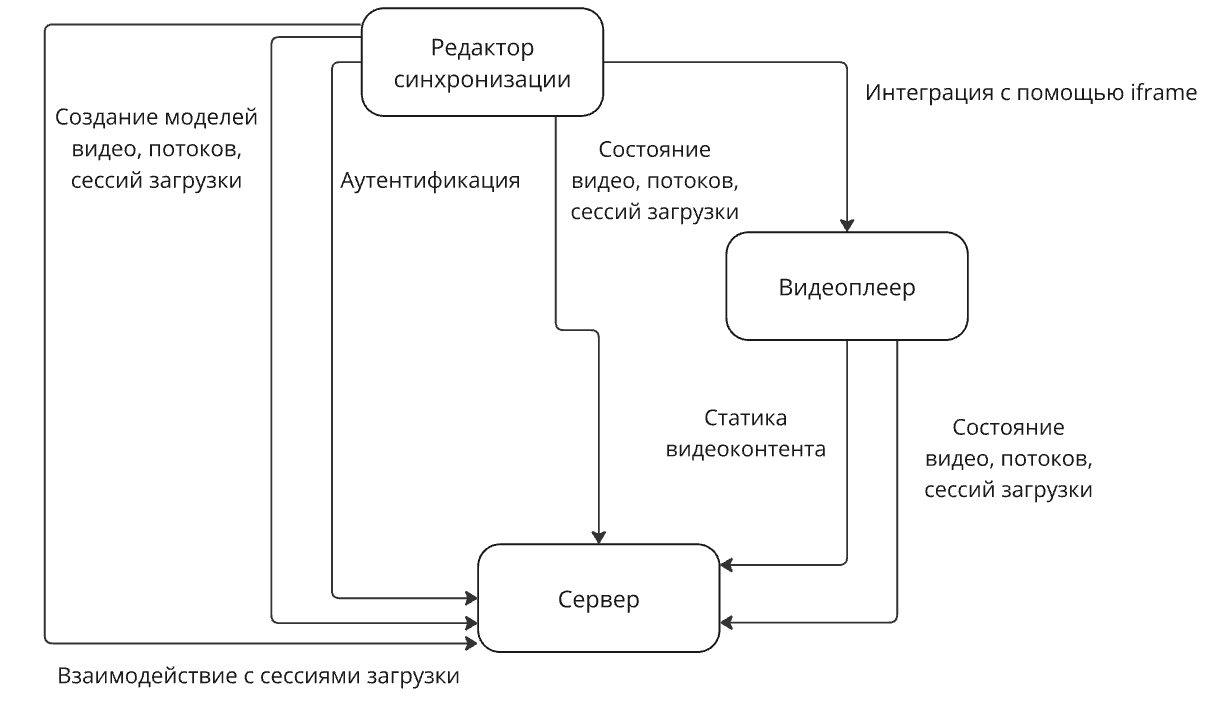
\includegraphics [scale=0.37] {my_folder/images//system_scheme_1}
		\caption{Схема системы первого уровня декомпозиции} 
		\label{fig:system_scheme_1}  
	\end{figure}

	Важно понимать, что высоконагруженные приложения не могут себе позволить использовать сервер одновременно и для выполнения какой-либо бизнес логики, и для раздачи статического контента. Это обусловлено тем, что часть своего процессорного времени сервер будет тратить также на передачу статики пользователю. В случае с видеоконтентом раздача его статического контента будет достаточно ресурсоемкой операцией. Необходимо какое-то разделение ответственности. Кроме того, в рассматриваемом проекте количество чтений статического контента будет сильно превышать количество записей, как в аналогичных системах. Эти доводы говорят о необходимости сепарирования логики загрузки и раздачи статического контента видео от головной части сервера. Теперь серверную часть можно представить в виде головного сервиса - API-Шлюза (API-Gateway), и сервиса загрузки и раздачи видео статики. Обновленная схема системы представлена на рисунке \ref{fig:system_scheme_2}.

	\begin{figure}[ht!] 
		\center
		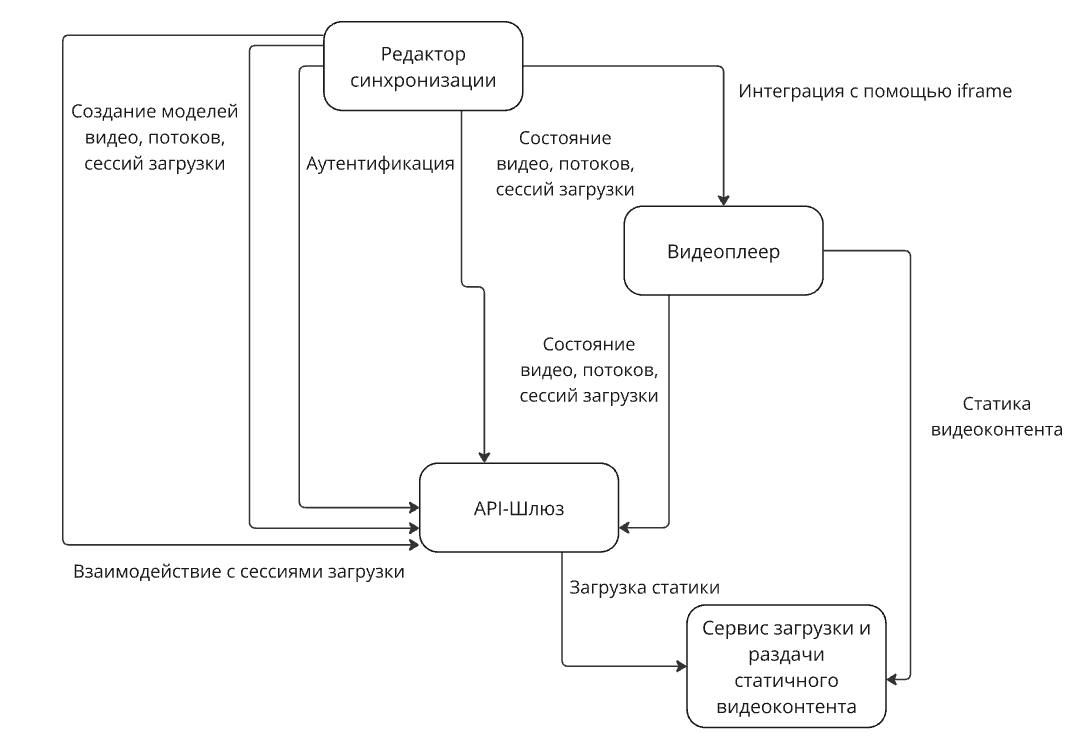
\includegraphics [scale=0.37] {my_folder/images//system_scheme_2}
		\caption{Схема системы второго уровня декомпозиции} 
		\label{fig:system_scheme_2}  
	\end{figure}
	
	 Среди перечисленных ранее требований к системе содержится доступность и отказоустойчивость. Обеспечение бесперебойной загрузки видеоконтента при нестабильной пропускной способности пользователя является нетривиальной задачей. При загрузке видео единым потоком трудно гарантировать его своевременную доставку и обработку, более того, длительность HTTP запросов ограничивают современные браузеры, принудительно их прерывая. Помимо прочего, для таких ресурсоемких обработок тяжело рассчитать допустимую нагрузку. Поэтому при проектировании архитектуры приложения оперировать абстрактными сущностями нет возможности, необходимо учитывать специфику. Одним из решений проблемы отказоустойчивости и доступности системы, которая должна обрабатывать большое количество бинарных данных, является сегментация контента, то есть разбиение его на сегменты или чанки. Они могут быть произвольной длины, однако для того, чтобы равномерно распределить нагрузку между клиентами, необходимо определить одинаковый размер для всех сегментов.

	Такое решение позволило рассматривать процесс загрузки видеоконтента не как "чёрный ящик", основную работу которого выполняет браузер и разработанные части серверных фреймворков, а как достаточно предсказуемую и контролируемую процедуру. Клиент сможет обрабатывать прерванные запросы и продолжать работу с сессиями загрузки, даже через несколько минут после восстановления сети или сервера.

	Можно заметить, что между сервисом-хранилищем статического видеоконтента и API-шлюзом есть незаполненное функциональное пространство, так как в API-шлюзе мы получаем необработанные бинарные данные в видео сегментов, а на сервисе-хранилище статики видео хранятся данные в виде закодированных чанков и объединяющих их манифестах HLS и MPEG-DASH. Это пространство должен занять транскодировщик, в зоне ответственности которого будет принять бинарные данные от API-Шлюза, преобразовать их в нужные форматы, аудио и видео кодеки, и загрузить на сервис со статикой.

	Однако располагать транскодировщик внутри головного сервиса является дорогостоящим и трудно масштабируемым решением, так как основная задача API-шлюза состоит в быстрой обработке пользовательских запросов, а транскодирование это сложная вычислительная задача. Как минимум структурно, даже не затрагивая возможности горизонтального масштабирования, транскодировщик должен располагаться отдельно. Обновленная схема системы с учетом транскодировщика представлена на рисунке \ref{fig:system_scheme_3}.
	\begin{figure}[ht!] 
		\center
		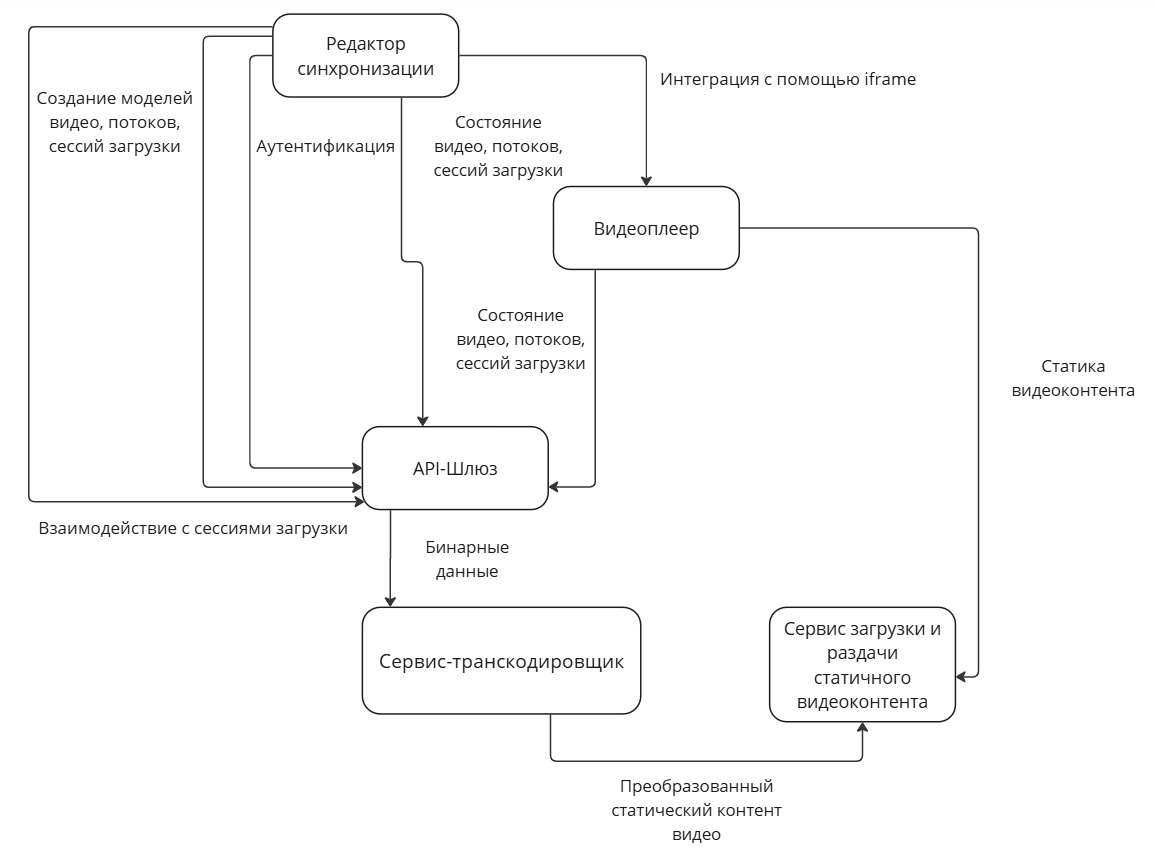
\includegraphics [scale=0.37] {my_folder/images//system_scheme_3}
		\caption{Схема системы третьего уровня декомпозиции} 
		\label{fig:system_scheme_3}  
	\end{figure}

\section{Техническая проработка системы} \label{ch2:technical_study}

	В этой части проектирования рассматриваются не только сами компоненты системы, но и способы организации взаимодействия между ними, а также состояния приложения, которые требуют хранения и отслеживания в базе данных для обеспечения консистентности данных и соблюдения бизнес-логики системы.

	Из рассмотренной ранее схемы приложения (рис. \ref{fig:system_scheme_3}) можно сделать вывод, что система точно содержит несколько состояний. Это говорит о необходимости использования базы данных для их хранения. На основе ранее описанных функциональных и нефункциональных требований можно выделить четыре сущности:
	\begin{itemize}[label=$\bullet$]
		\item Пользователь;
		\item Видео;
		\item Поток;
		\item Сессия загрузки.
	\end{itemize}

	Пользователь (User) необходим для того, чтобы по загруженному в систему контенту можно было идентифицировать его создателя. Кроме того, пользователи должны иметь разграничение доступа к контенту - только создатели видео могут взаимодействовать с сессиями загрузки. Экземпляр пользователя должен содержать идентификатор, email - для возможного продуктового масштабирования в будущем (отправка писем на почту, двухфакторная аутентификация), хеш пароля - для аутентификации, дату регистрации.

	Видео (Video) представляет собой абстрактную сущность, которая содержит идентификатор, заголовок, описание, дату создания, дату полной загрузки и ссылку на пользователя-создателя, а также текущий статус видео. Статус включает следующие состояния:
	\begin{itemize}[label=$\bullet$]
		\item Создано (CREATED);
		\item Загружается (UPLOADING);
		\item Раздаётся (DISTRIBUTED);
		\item Заблокировано (BLOCKED).
	\end{itemize}

	Каждое видео может содержать множество связанных с ним потоков, которые будут отображаться в плеере.

	Поток (Flow), как сущность, похож на видео, однако содержит специфичную информацию о конкретном потоке, который будет воспроизводиться в плеере. Он содержит индентификатор, текущий статус, дату создания, дату загрузки, ссылку на привязанное к потоку видео. Статус включает следующие состояния:
	\begin{itemize}[label=$\bullet$]
		\item Создано (CREATED);
		\item Загружается (UPLOADING);
		\item Раздаётся (DISTRIBUTED);
		\item Скрыт (HIDDEN).
	\end{itemize}

	Каждый поток может содержать сессию загрузки, но притом только одну. К потоку может быть привязана сессия загрузки тогда и только тогда, когда его статус равен "Загружается".

	Благодаря сессии загрузки пользователи могут отслеживать процесс загрузки каждого потока в отдельности. Кроме того, сессия позволяет поддерживать консистентность загрузки и обработки видеоконтента, чтобы система была устойчива к "промахам" при загрузке видео со стороны пользователей. Она должна содержать идентификатор, что полезно также для логирования и отслеживания промежуточных состояний загрузки для стороны разработки, общее количество байт потока, количество уже загруженных и обработанных байтов видео, ссылку на связанный поток.
	
	Данные имеют чёткие структуру и связи между собой, что говорит о необходимости использования реляционной базы данных для их хранения.

	Для хранения данных системы были созданы соответствующие таблицы с необходимыми столбцами и типами. Схема таблиц представлена на рисунке \ref{fig:db_scheme}.
	\begin{figure}[ht!] 
		\center
		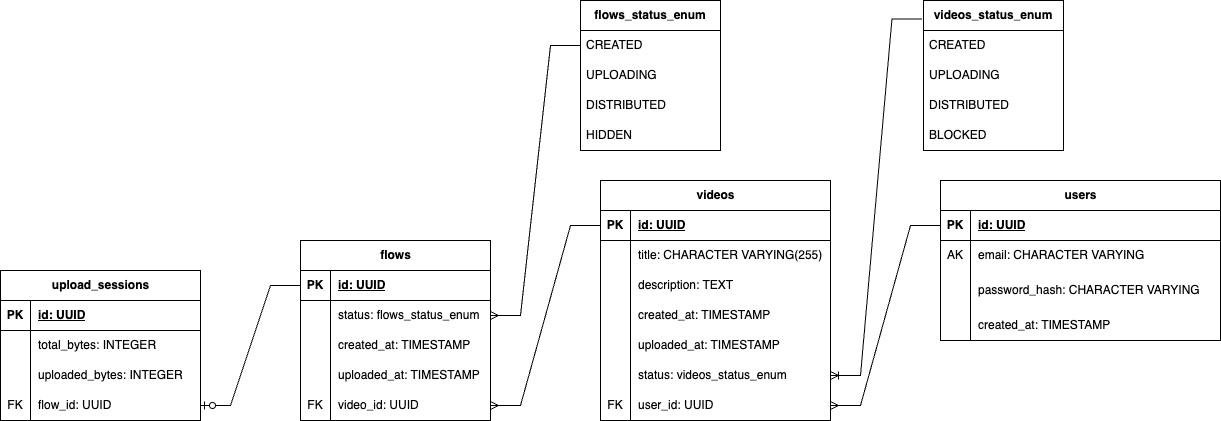
\includegraphics [scale=0.37] {my_folder/images//db_scheme}
		\caption{Схема таблиц базы данных системы} 
		\label{fig:db_scheme}  
	\end{figure}

	При загрузке видео, разделённого на сегменты, последовательно, без задержек существенно возрастет нагрузка на сервис-транскодировщик. Помимо того, что сама операция транскодирования является ресурсоёмкой, количество одновременных сессий загрузки может быть большим. API-шлюз должен отвечать на запросы пользователей как можно скорее и позволить ему дождаться результата выполнений транскодирования, проводить валидацию отправленных сегментов нет возможности, так как это ухудшит пользовательский опыт.

	Чтобы решить эту проблему, головному сервису необходимо возвращать ответ пользователю синхронно, а саму обработку осуществлять асинхронно. Для решения задач подобного рода используются брокеры сообщений или очереди, которые позволяют упорядочить задачи для выполнения в единую структуру типа FIFO.

	Однако при такой реализации API-Шлюзу необходимо предусмотреть возможность отслеживания состояния загрузки видео для клиента. Эта проблема может быть решена различными способами: поллингом состояния или оповещением клиента о его изменении с помощью технологии WebSocket. Но главное, что при таком способе решения проблемы единственным источником истины является состояние в базе данных, а способ обработки данных не имеет значения.

	Обновленная схема системы с учетом новых сущностей представлена на рисунке 5.

	\begin{figure}[ht!] 
		\center
		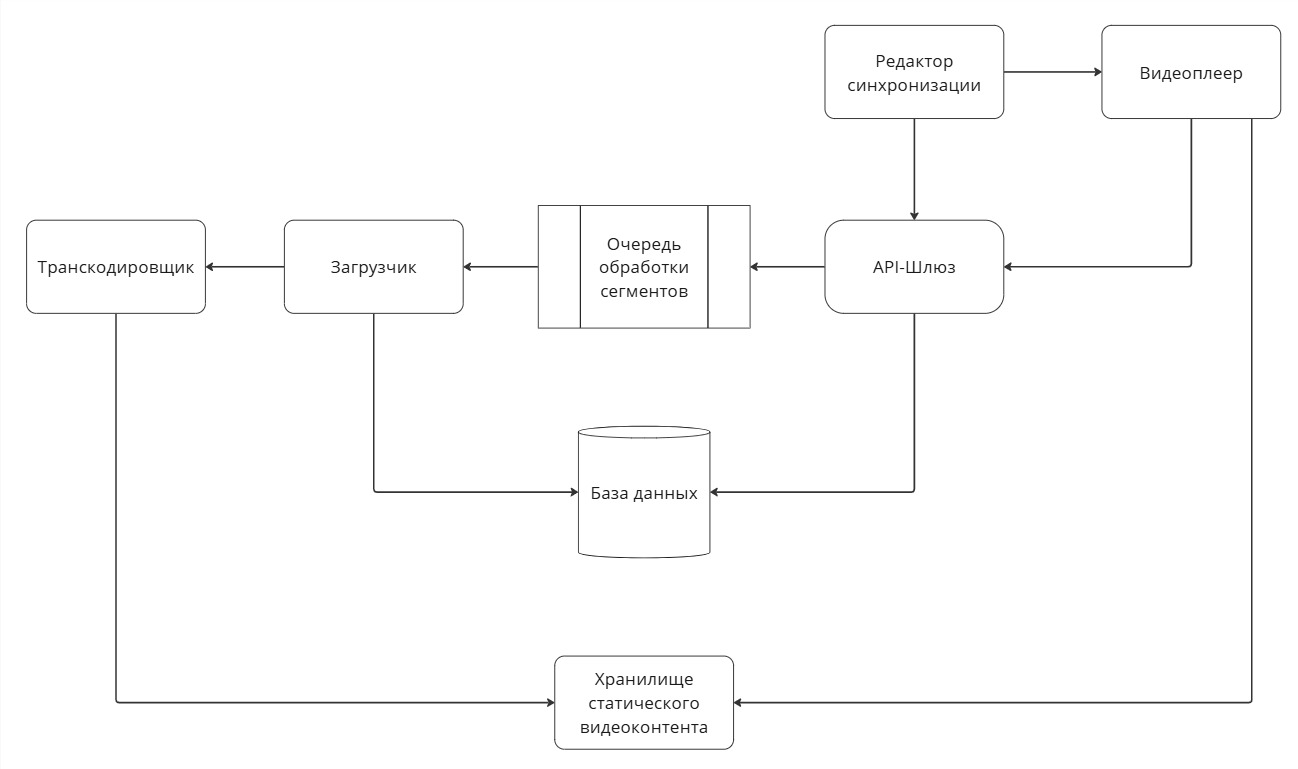
\includegraphics [scale=0.33] {my_folder/images//system_scheme_4}
		\caption{Схема системы c учётом базы данных, очереди обработки видеосегментов и сервисом-загрузчиком} 
		\label{fig:system_scheme_4}  
	\end{figure}

	Важно уточнить, что в системе также должен быть предусмотрен и механизм очищения созданных и неиспользуемых сессий загрузки и видео, так как, помимо лишней информации в базе данных, создаются дополнительные ресурсы в сервисе-транскодировщике, и при их неконтролируемом росте система теряет всякую возможность масштабирования. Для решения проблем такого рода используются планировщики задач (англ. job scheduler). Планировщик с определённой периодичностью выполняет часть бизнес логики приложения, которая требует периодичности, а затем прекращает свою работу. В текущем проекте планировщику необходимо периодически уничтожать неиспользуемые сессии как ресурс в транскодировщике, так и информацию о них и связанных сущностях в базе данных. Соответственно, такая функциональность структурно должна быть расположена где-то между сервисом-загрузчиком и сервисом-транскодировщиком, если исходить из схемы системы. Запуск планировщик как отдельный процесс операционный системы является дорогим решением, так как требует дополнительных ресурсов на среду выполнения и ещё одно подключение к базе данных. Поэтому оптимальным решением будет расположить логику работы планировщика внутри сервиса-загрузчика, так как он будет содержать пул соединений к базе данных, а также иметь программную реализацию коммуникации с сервисом-транскодировщиком. В таком случае при выборе технологии для реализации сервиса-загрузчика необходимо отталкиваться от возможности планирования задач.

\section{Инструменты реализации компонентов системы}

	Теперь, когда структура системы определена и включены все основные компоненты, необходимо перейти к выбору технологий для реализации сервисов. В рамках данного этапа будут определены инструменты и программные средства для реализации сервисов системы, их масштабирования и безопасности, а также средства коммуникации между ними. Для это рассмотрим особенности каждого из сервисов и определим соответствующие технологии.

	\subsection{Выбор СУБД}

	Для реализации серверной части системы необходима система управления базами данных, предназначенная для хранения пользовательских данных и информации о состоянии сущностей: видео, потоков и сессий загрузки. СУБД должна быть реляционной, так как для данных, которые планируется хранить, важны структурированность, чёткая схема и возможность эффективного выполнения сложных запросов и выборок с использованием соединений. Также обязательным требованием является поддержка многопоточной работы и транзакционности, так как доступ к данным будет осуществляться в нескольких потоках.

	Из решений с открытым исходным кодом таким требованиям в наибольшей степени соответствует PostgreSQL. Эта СУБД обладает развитой поддержкой транзакций, гарантирует целостность и изолированность данных даже при высокой конкуренции потоков и процессов. Кроме того, PostgreSQL содержит в себе возможность шардирования (техника горизонтального разделения больших баз данных на более мелкие) базы данных, что позволяет масштабировать систему в будущем.

	\subsection{Выбор брокера сообщений}

	Для эффективной реализации асинхронной обработки сегментов необходимо использовать брокер сообщений. Основными требованиями к брокеру являются: надёжная доставка сообщений, подтверждение очереди о принятии сообщений, а также гарантия согласованности данных в случае отказов или временной недоступности отдельных компонентов. Важность перечисленных требований объясняется тем, что сегменты видео содержат определённый порядок, и даже потеря одного из них приведёт к повреждённому видео.

	Из решений с открытым исходным кодом указанным наиболее полно соответствует требованиям брокер RabbitMQ. RabbitMQ использует стандартный протокол AMQP и предоставляет встроенные механизмы подтверждения принятия сообщений и повторной отправки в случае сбоев, что позволяет гарантировать доставку и сохранять согласованность данных во всех асинхронных сценариях системы.

	\subsection{Выбор инструментов для реализации API-Шлюза}
	
	API-шлюз – это основная точка входа в систему, которая обеспечивает маршрутизацию запросов, аутентификацию пользователей, управление сессиями и доступ к состоянию видео, потоков, сессий. Ключевая задача API-шлюза – возвращать результат пользователю как можно быстрее, минимизируя задержки при обработке запросов, чтобы не блокировать пользовательские сценарии. Для этого он не ждет завершения длительных операций, таких как транскодирование, а выполняет обработку асинхронно, передавая задачи в очередь RabbitMQ, и возвращает пользователю подтверждение о приеме данных, а также формирует ссылки на статические файлы видеоконтента. Взаимодействие с сервисом происходит посредством HTTP. Характеристика сервиса выше говорит о том, что Node.js будет оптимальным выбором для API-шлюза, поскольку его неблокирующий ввод/вывод позволяет эффективно обрабатывать большое количество одновременных запросов без создания дополнительных потоков, что значительно снижает нагрузку на сервер и позволяет без проблем масштабироваться горизонтально, также учитывая, что многие модули Node.JS написаны на низкоуровневых языках программирования.

	\subsection{Выбор инструментов для реализации сервиса-загрузчика}

	Сервис-загрузчик отвечает за прием поступающих сегментов видео, их валидацию, отправку на транскодирование, а также управление сессиями загрузки, включая их удаление после истечения срока хранения, и обновление состояния видео, потоков, сессий, включая отслеживание их консистентности. Он должен поддерживать обработку бинарных данных, интегрироваться с брокером сообщений для принятия задач, а также иметь высокую производительность, так как является самым нагруженным по части бизнес-логики. Также сервис включает планировщик, который автоматически удаляет неиспользуемые или просроченные сессии загрузки, освобождая ресурсы и поддерживая актуальность данных. Java является оптимальным выбором, так как поддерживает многопоточность и оптимальный баланс между уровнем абстракции и производительностью языка. В качестве фреймворка лучше всего использовать Spring Boot, который предоставляет удобные механизмы для интеграции с RabbitMQ. Этот фреймворк также содержит удобный механизм для периодического выполнения задач - Spring Task Scheduler, который позволяет эффективно управлять автоматическими процессами без нагрузки на основные бизнес-операции.
	
	\subsection{Выбор инструментов для реализации сервиса-транскодировщика}
	
	Сервис-транскодировщик отвечает за обработку, транскодирование загруженных сегментов видео, объединение их в полноценное видео, которое состоит из статического контента: манифестов для потокового вещания в форматах HLS и MPEG-DASH и соответствующих чанков, а также отправку полученных файлов на сервис-хранилище через FTP. Сервис и принадлежащие ему процессы управляемы извне посредством HTTP. В основе сервиса должен быть непосредственно транскодировщик. Оптимальным выбором в данной связи будет FFmpeg – мощное средство кодирования и транскодирования видео, которое является стандартом и фактически монополистом в области мультимедийной обработки, предоставляя поддержку всех популярных кодеков, контейнеров и форматов трансляции. Благодаря неблокирующему вводу/выводу (Non-blocking I/O) в Node.js, сервис может одновременно обрабатывать и передавать по FTP большое количество файлов, не блокируя выполнение других задач. Это позволяет масштабировать транскодирование.

	\subsection{Выбор инструментов для реализации сервиса-хранилища статического видеоконтента}

	Сервис-хранилище статического видеоконтента отвечает за прием транскодированных видеофайлов через FTP и их раздачу пользователям по HTTP. Он также должен обеспечивать быструю обработку нескольких запросов одновременно. Как в случае с API-Шлюзом, неблокирующий ввод/вывод, поддерживаемый по умолчанию в Node.JS, выделяет его как оптимальное средство для соблюдения поставленных требований. А в совокупности с Express.js позволяет поддержать раздачу статического контента без дополнительных настроек.

	\subsection{Выбор инструментов для реализации клиентских приложений}

	Клиентские приложения могут быть разработаны только на JavaScript, поскольку это единственный язык программирования, поддерживаемый всеми современными и устаревшими браузерами. Видеоплеер и редактор синхронизации характеризуются большим количеством динамических состояний и асинхронных операций, что повышает риск возникновения ошибок. Для снижения вероятности ошибок приложение должно основываться на иммутабельности данных и использовать эффективный менеджер асинхронных операций и событий. Таким требованиям соответствует набор инструментов React, Redux и Redux-Saga, которые позволяют выстраивать масштабируемую древовидную структуру: React – компонентов, Redux – состояния, Redux-Saga – событий. React обеспечивает компонентную архитектуру и декларативный подход, Redux управляет состоянием на основе иммутабельности, а Redux-Saga эффективно управляет асинхронными операциями на основе генераторов и собственного менеджера.

	Обновленная схема системы с учётом всех выбранных технологий и протоколов коммуникации представлена на рисунке \ref{fig:system_scheme_5}.
	\begin{figure}[ht!] 
		\center
		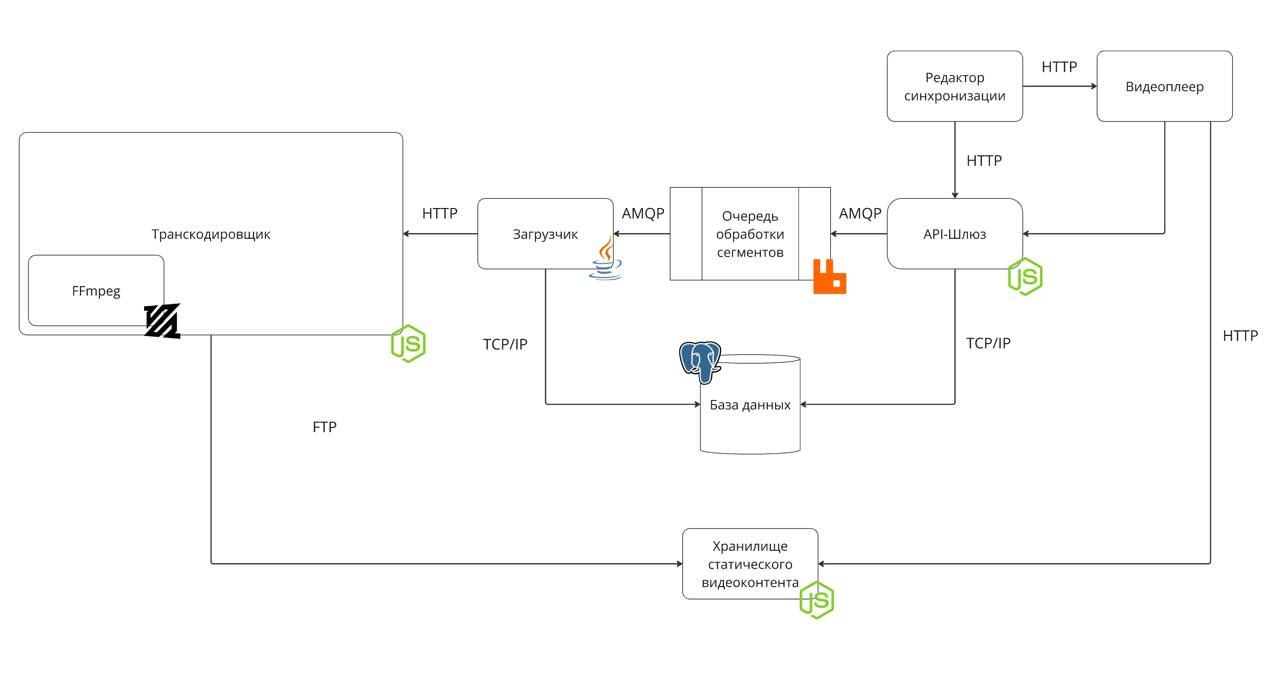
\includegraphics [scale=0.35] {my_folder/images//system_scheme_5}
		\caption{Схема системы c учётом выбранных технологий} 
		\label{fig:system_scheme_5}  
	\end{figure}

	\subsection{Выбор инструмента балансировки нагрузки}

	Несмотря на все описанные выше оптимизации и разграничения ответственности, риск выхода из строя всей системы всё равно есть. Если один из сервисов не справится с нагрузкой и резко прекратит работу, система, как минимум, перестанет работать ожидаемо. Даже при обработке всех возможных ошибок в сервисах такая вероятность никогда не равняется нулю. Чтобы минимизировать эти риски, необходимо реплицировать существующие сервисы. В таком случае при выходе из строя одного из них остальные будут работать, как и прежде, а его нагрузку распределят между собой остальные сервисы. Однако при таком подходе необходим механизм, который бы принимал все запросы от клиента сервиса и распределял трафик между такими репликациями. Для решения этой задачи необходимо использовать балансировщик нагрузки. Лидером среди них является NGINX, который также является и решением с открытым кодом. В текущем проекте балансировщик может быть использован для каждого сервиса, который будет содержать открытый порт для коммуникации с ним.
	
	Под это описание подходят все сервисы, кроме загрузчика. Его можно реплицировать без добавления балансировщика нагрузки, так как каждая реплика будет читать сообщения из очереди независимо. Однако важно учитывать, что в таком случае, каждая реплика этого сервиса не должна содержать планировщик, который очищает ресурсы просроченной сессии. Планировщика достаточно расположить на одной стандалон-реплике (англ. standalone). Чтобы это сделать, необходимо реализовать инициализацию планировщика на основе значения переменной окружения. В таком случае мы сможем регулировать планировщик и реплику его запуска.

	\subsection{Выбор инструмента кэширования}

	Ещё одна проблема может возникнуть с реплицированием сервиса-транскодировщика, так как он порождает процессы FFmpeg, которые привязаны к конкретной реплике. Это значит, что после запроса на создание процесса транскодирования для какой-то сессии загрузки, все последующие запросы должны маршрутизироваться на конкретную реплику транскодировщика. Кроме того, реплики сервиса-загрузчика равномерно между собой будут распределять задачи из очереди. Это значит, что разные реплики загрузчика могут работать с одинаковыми сессиями и необходимо синхронизировать между ними маршрутизацию до определенной реплики транскодировщика. Для решения этой проблемы необходимо использовать сервис для кэширования типа “Ключ=Значение”, чтобы реплики могли делиться между собой информацией о маршруте до нужной реплики. Лидером среди таких решений, является СУБД Redis. Помимо прочего, такая маршрутизация требует и дополнительной настройки со стороны NGINX, которую тоже необходимо предусмотреть.
	
	Схема системы с учётом необходимости реплицирования и балансировки нагрузки представлена на рисунке \ref{fig:system_scheme_6}.

	\begin{figure}[ht!] 
		\center
		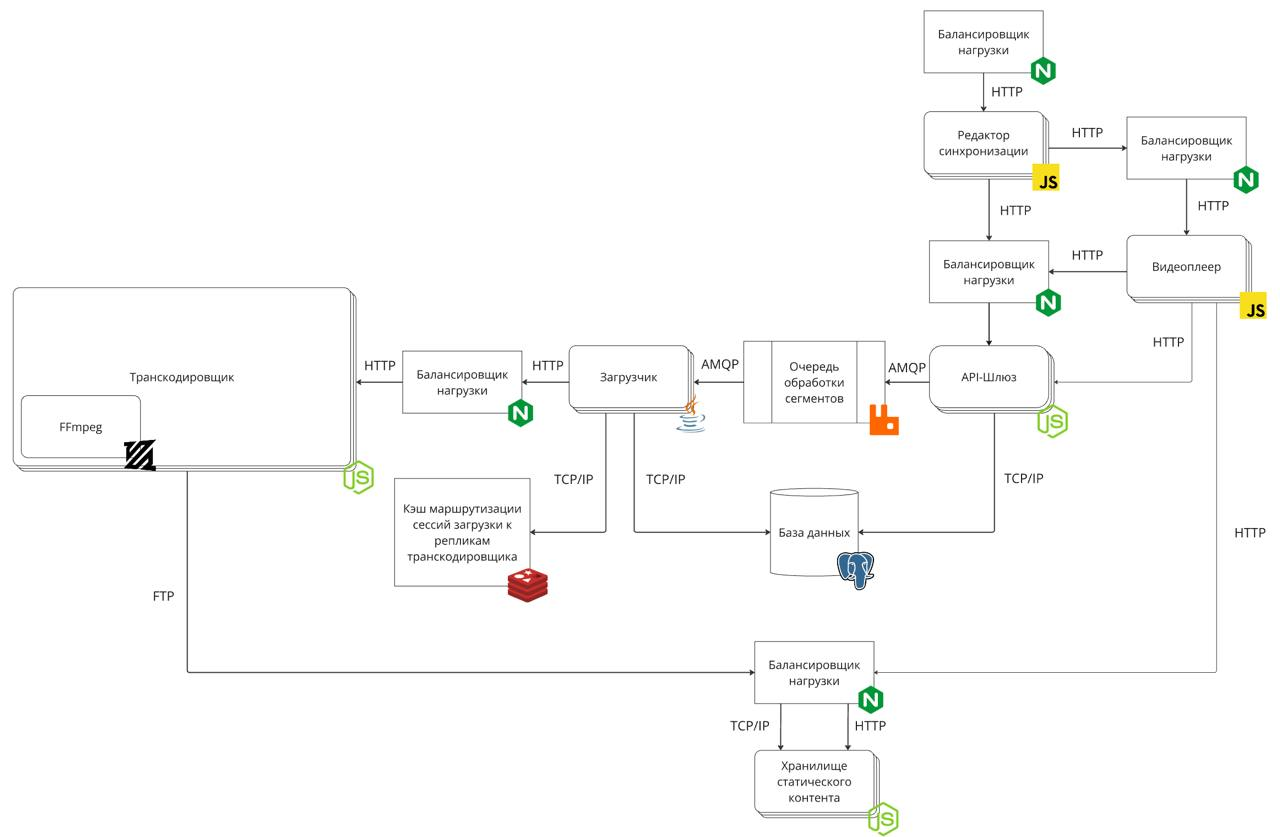
\includegraphics [scale=0.32] {my_folder/images//system_scheme_6}
		\caption{Схема системы c учётом инструментов кэширования и балансировки нагрузки} 
		\label{fig:system_scheme_6}  
	\end{figure}

	\subsection{Обеспечение безопасности межсервисной сетевой коммуникации}

	Важно учитывать, что при такой реализации без дополнительного конфигурирования и разработки будет огромное количество открытых TCP/IP портов, что не является безопасным. Для того, чтобы решить эту проблему, необходимо создать приватную сеть для межсервисного взаимодействия и оставить открытыми только те порты, на которые клиент может безопасно отправлять запросы. Разделим на схеме стрелки, определяющие межсервисную коммуникацию, по признаку приватности/публичности на основе цвета. Обновлённая схема представлена на рисунке \ref{fig:system_scheme_7}.

	\begin{figure}[ht!] 
		\center
		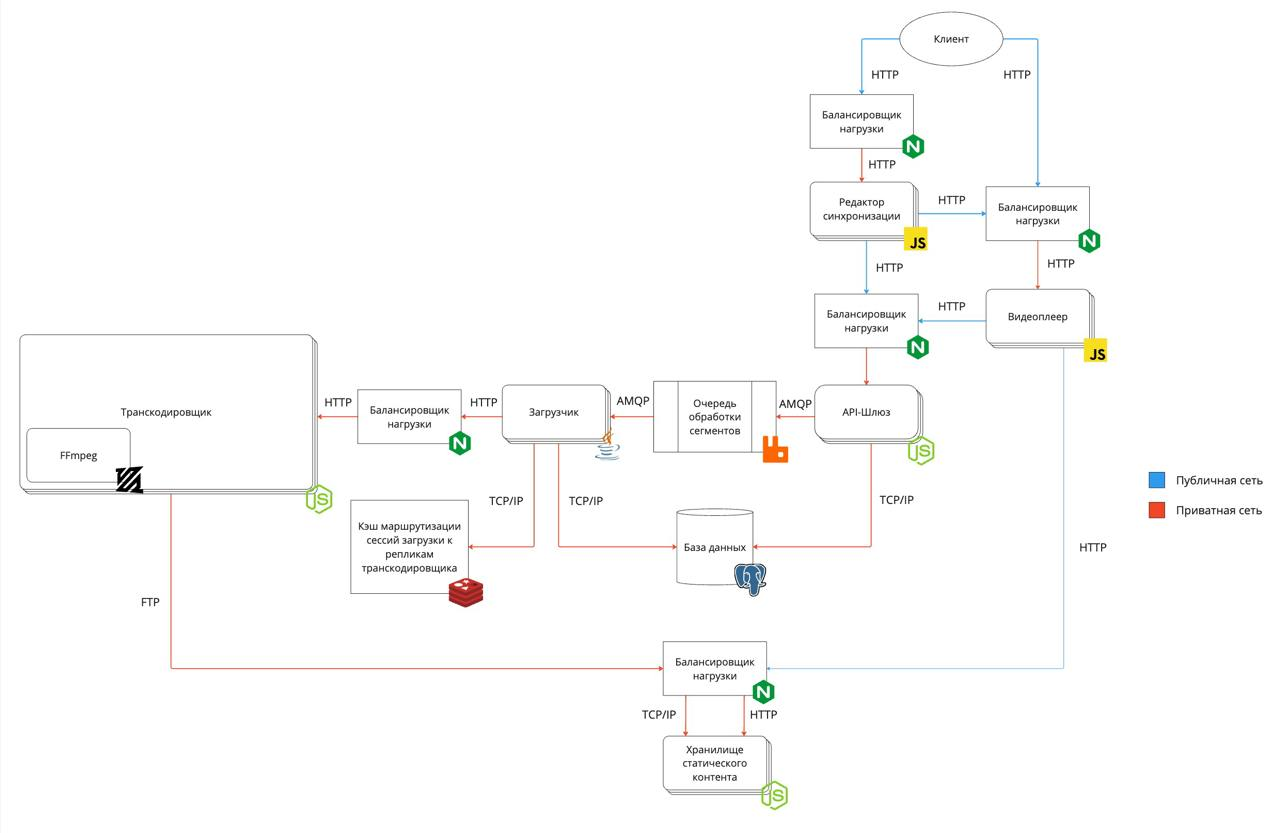
\includegraphics [scale=0.32] {my_folder/images//system_scheme_7}
		\caption{Схема системы c учётом безопасности межсервисной сетевой коммуникации} 
		\label{fig:system_scheme_7}  
	\end{figure}
	
\section{Выводы}

	В данной главе разработана архитектура системы распределённой сегментированной загрузки и раздачи видеоконтента. Формирование архитектурных решений было основано на анализе требований к масштабируемости, отказоустойчивости, адаптивности системы к нагрузке и обеспечению бесперебойного взаимодействия пользователей с приложением. В ходе проектирования были выделены основные функциональные компоненты системы. определены методы взаимодействия между компонентами, механизмы асинхронной обработки данных, способы передачи видеоконтента и оптимальные технологии для реализации каждого сервиса, а также определены способы и технологии для балансирования нагрузки между ними и поддержания безопасности при межсервисном взаимодействии.
	
